\documentclass[aspectratio=169,11pt]{beamer}
\usetheme{metropolis}
\usepackage{booktabs,graphicx,amsmath}
\setbeamertemplate{frame numbering}[fraction]
\definecolor{acc}{HTML}{2A78D6}
\setbeamercolor{alerted text}{fg=acc}
\newcommand{\rmpp}{ReMasker++}
\newcommand{\remasker}{ReMasker}
\graphicspath{{../results/figures/}}

\title{ReMasker++: Missingness-Aligned Masked Autoencoding\\with Learned Uncertainty for Tabular Imputation}
\subtitle{MA 305: Data Science --- End-Term Evaluation}
\author{\small Team 2: Jandhyala Mohana Sarath Chandra (240041020)\\ Aayush Sharma (240041001) \quad Arnav Nitin Birari (240041004)}
\institute{Instructor: Prof.\ M.\ Tanveer \hfill \texttt{github.com/sunno-bhaato/remasker\_pp}}
\date{November 2026}

\begin{document}
\maketitle

\begin{frame}{From reproduction to a new method}
\begin{columns}[T]
\column{0.5\textwidth}
\textbf{Mid-eval:} reproduced ReMasker (ICLR'24) on Yacht.\\[6pt]
\textbf{Now:} we \alert{designed, built and benchmarked} \rmpp, which targets the limitations the ReMasker authors state themselves.
\column{0.5\textwidth}
\small
\begin{tabular}{p{0.45\linewidth}p{0.45\linewidth}}
\toprule
\textbf{ReMasker limitation} & \textbf{\rmpp{} fix}\\\midrule
Re-masks $\ne$ real missingness (MCAR$\to$MNAR gap) & Missingness-aligned re-masking\\
No idea which imputations to trust & Learned per-cell uncertainty\\
Good RMSE, worse WD & Wasserstein loss (W)\\
Row-by-row inference & Batched equivalent model\\\bottomrule
\end{tabular}
\end{columns}
\end{frame}

\begin{frame}{Where the field is (2024--2026)}
\begin{itemize}
\item \textbf{ReMasker} (ICLR'24): masked autoencoder; re-mask random observed cells, reconstruct them.
\item \textbf{CACTI} (ICML'25): copy-masking + LLM column context. \textbf{PMAE} ('24): proportional masking.
\item \textbf{DiffPuter} (ICLR'25), \textbf{RefiDiff} (AAAI'26): diffusion-based imputers.
\item \textbf{TabImpute} ('25): zero-shot TabPFN-style foundation model.
\item Strong classical baseline: \textbf{HyperImpute} (ICML'22, auto-tuned iterative ensemble).
\end{itemize}
\vspace{4pt}
\alert{Our angle:} keep ReMasker's simple single model, fix its training signal, and add \emph{uncertainty}, which none of the masked-autoencoder imputers provide.
\end{frame}

\section{Method}

\begin{frame}{Idea 1: Missingness-aligned re-masking}
\begin{columns}[T]
\column{0.55\textwidth}
\textbf{ReMasker:} hide a \emph{uniformly random} 50\% of observed cells and learn to reconstruct them.\\[4pt]
\textbf{Problem:} at test time the hidden cells follow the \emph{real} missingness mechanism, which is structured (MAR/MNAR).\\[4pt]
\textbf{\rmpp:} for row $i$, borrow the real missing pattern $M_j$ of a random row $j$:
\[ R_i = O_i \cap M_j,\qquad V_i = O_i\setminus M_j \]
so the \alert{training task matches the test task}.
\column{0.42\textwidth}
\small
\begin{tabular}{lcccc}
 & $x_1$ & $x_2$ & $x_3$ & $x_4$\\\midrule
row $i$ & 0.3 & 0.7 & \textbf{?} & 0.1\\
donor $j$ & 0.5 & \textbf{?} & 0.2 & \textbf{?}\\\midrule
train on $i$ & 0.3 & \alert{[M]} & \textbf{?} & \alert{[M]}\\
\end{tabular}\\[6pt]
\footnotesize Encoder sees $x_1$; loss on $x_2,x_4$.\\ Control: random masking at the same ratio (30\%).
\end{columns}
\end{frame}

\begin{frame}{Idea 2: Learned per-cell uncertainty (no accuracy cost)}
\begin{itemize}
\item Small MLP head $g_\phi$ on \alert{stop-gradient} decoder features predicts $s_k=\log\sigma_k^2$.
\item Trained on re-masked cells (ground truth known!) with a Gaussian NLL, mean detached:
\[\mathcal{L}_{\text{unc}}=\tfrac{1}{|R|}\textstyle\sum_{k\in R}\big[s_k+(x_k-\operatorname{sg}(\hat x_k))^2e^{-s_k}\big]\]
\item Optimum: $e^{s_k}=\mathbb{E}[(x_k-\hat x_k)^2\mid\text{context}]$, i.e.\ \alert{expected error of this imputation}.
\item No gradient reaches the imputer, so the \alert{imputations are unchanged}.
\end{itemize}
\textbf{Idea 3 (variant W):} add $\lambda\cdot$ exact 1-D Wasserstein loss per feature (sort and compare) to fight MSE's variance shrinkage.\\
\textbf{Engineering:} attention key-padding masks give the same model as token dropping, but batched.
\end{frame}

\section{Experiments}

\begin{frame}{Setup}
\begin{itemize}
\item \textbf{5 datasets}: yacht, airfoil, compression (regression); raisin, wine (classification).
\item \textbf{MCAR / MAR / MNAR} at 30\%, \textbf{3 seeds}: 45 runs per method.
\item \textbf{Baselines}: official ReMasker (same budget), HyperImpute, MissForest, MICE, GAIN, MIWAE, Sinkhorn, SoftImpute, Mean.
\item \textbf{Metrics}: RMSE, WD (fidelity); XGBoost + linear-model AUROC / $R^2$ vs.\ a complete-data oracle (utility); Spearman(uncertainty, error).
\item \textbf{Ablation} of 6 components, plus an MNAR stress test up to 70\% missing.
\end{itemize}
\end{frame}

\begin{frame}{Ablation: what actually helps}
\centering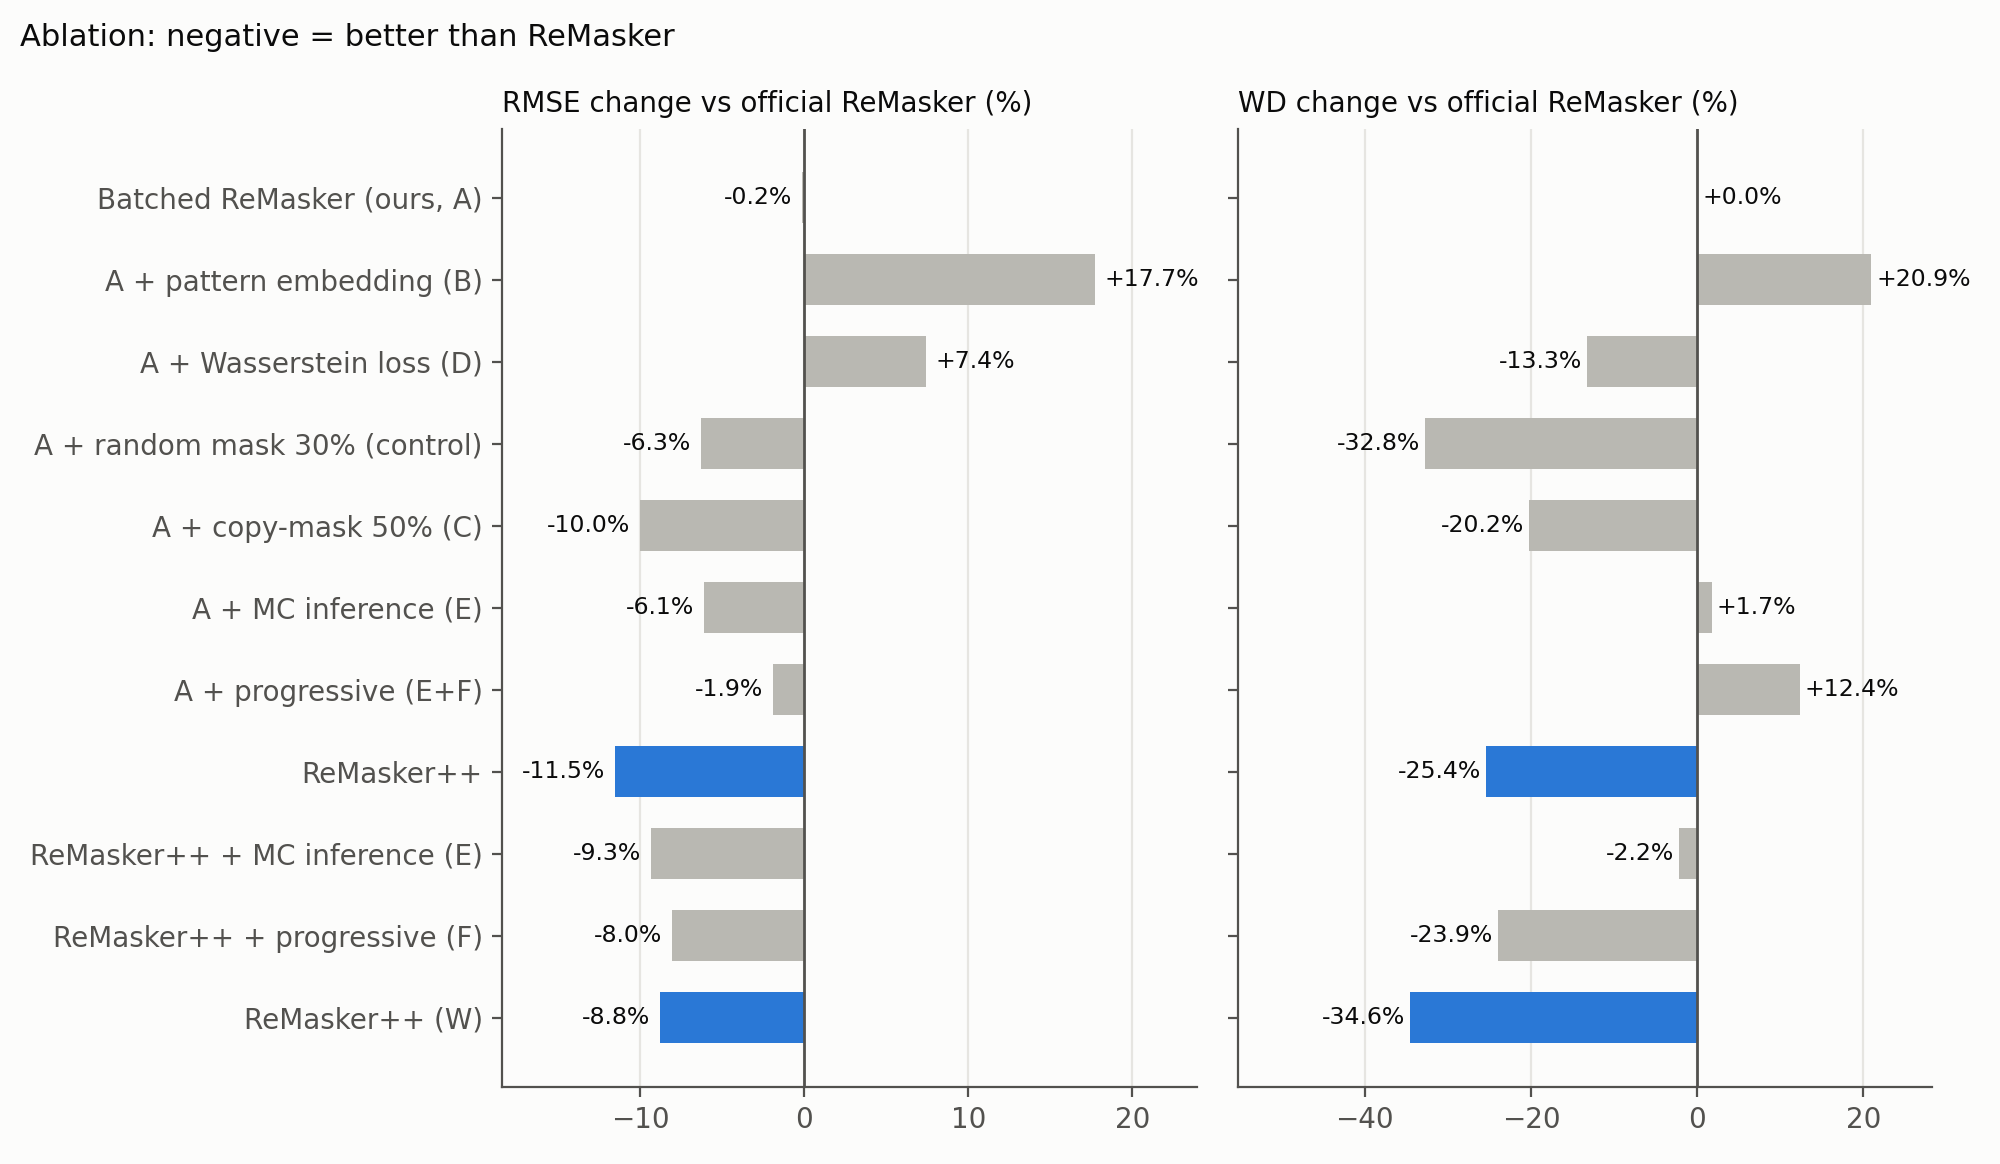
\includegraphics[height=0.82\textheight]{ablation.png}
\end{frame}

\begin{frame}{Ablation: takeaways}
\begin{itemize}
\item Our batched re-implementation matches official ReMasker ($-0.2\%$ RMSE) and its inference is \alert{$6\times$ faster}.
\item \alert{Missingness-aligned re-masking is the main driver}: $-11.5\%$ RMSE, $-25\%$ WD.
\item \textbf{Control}: random masking at the same 30\% ratio gives only $-6.3\%$ RMSE ($-3.9\%$ under MNAR vs.\ $-9.7\%$). About half the gain comes from \alert{realistic mask structure}.
\item Wasserstein loss: WD $-13\%$ alone; \rmpp{}\,(W) reaches \alert{$-34.6\%$ WD}.
\item Uncertainty head: \alert{no accuracy cost}, as designed.
\end{itemize}
\end{frame}

\begin{frame}[shrink=5]{Benchmark against established imputers}
\centering
\resizebox{0.92\linewidth}{!}{\begin{tabular}{lcccccc}
\toprule
Method & \multicolumn{3}{c}{RMSE $\downarrow$} & \multicolumn{3}{c}{WD $\downarrow$}\\
 & MCAR & MAR & MNAR & MCAR & MAR & MNAR\\
\midrule
\rmpp{} & \underline{0.1558} & \underline{0.1531} & \underline{0.1613} & 0.0594 & 0.0582 & 0.0643\\
\rmpp{} (W) & 0.1607 & 0.1604 & 0.1660 & \textbf{0.0510} & \underline{0.0520} & \underline{0.0568}\\
\remasker{} (official) & 0.1712 & 0.1752 & 0.1778 & 0.0725 & 0.0875 & 0.0737\\
\midrule
HyperImpute & \textbf{0.1512} & \textbf{0.1379} & \textbf{0.1569} & 0.0554 & \textbf{0.0520} & \textbf{0.0526}\\
MissForest & 0.1680 & 0.1738 & 0.1716 & 0.0838 & 0.0936 & 0.0866\\
MICE & 0.2375 & 0.2232 & 0.2448 & \underline{0.0546} & 0.0522 & 0.0597\\
\bottomrule
\end{tabular}
}\\[4pt]
\small RMSE / WD at 30\% missing, average over 5 datasets $\times$ 3 seeds. \textbf{Best}, \underline{2nd}.\\[4pt]
\normalsize \rmpp{} beats official ReMasker and MissForest in \alert{15/15 settings on RMSE and WD}.\\ Against HyperImpute: wins 6/15 settings on RMSE and 6/15 on WD.
\end{frame}

\begin{frame}{Average rank across 15 settings}
\centering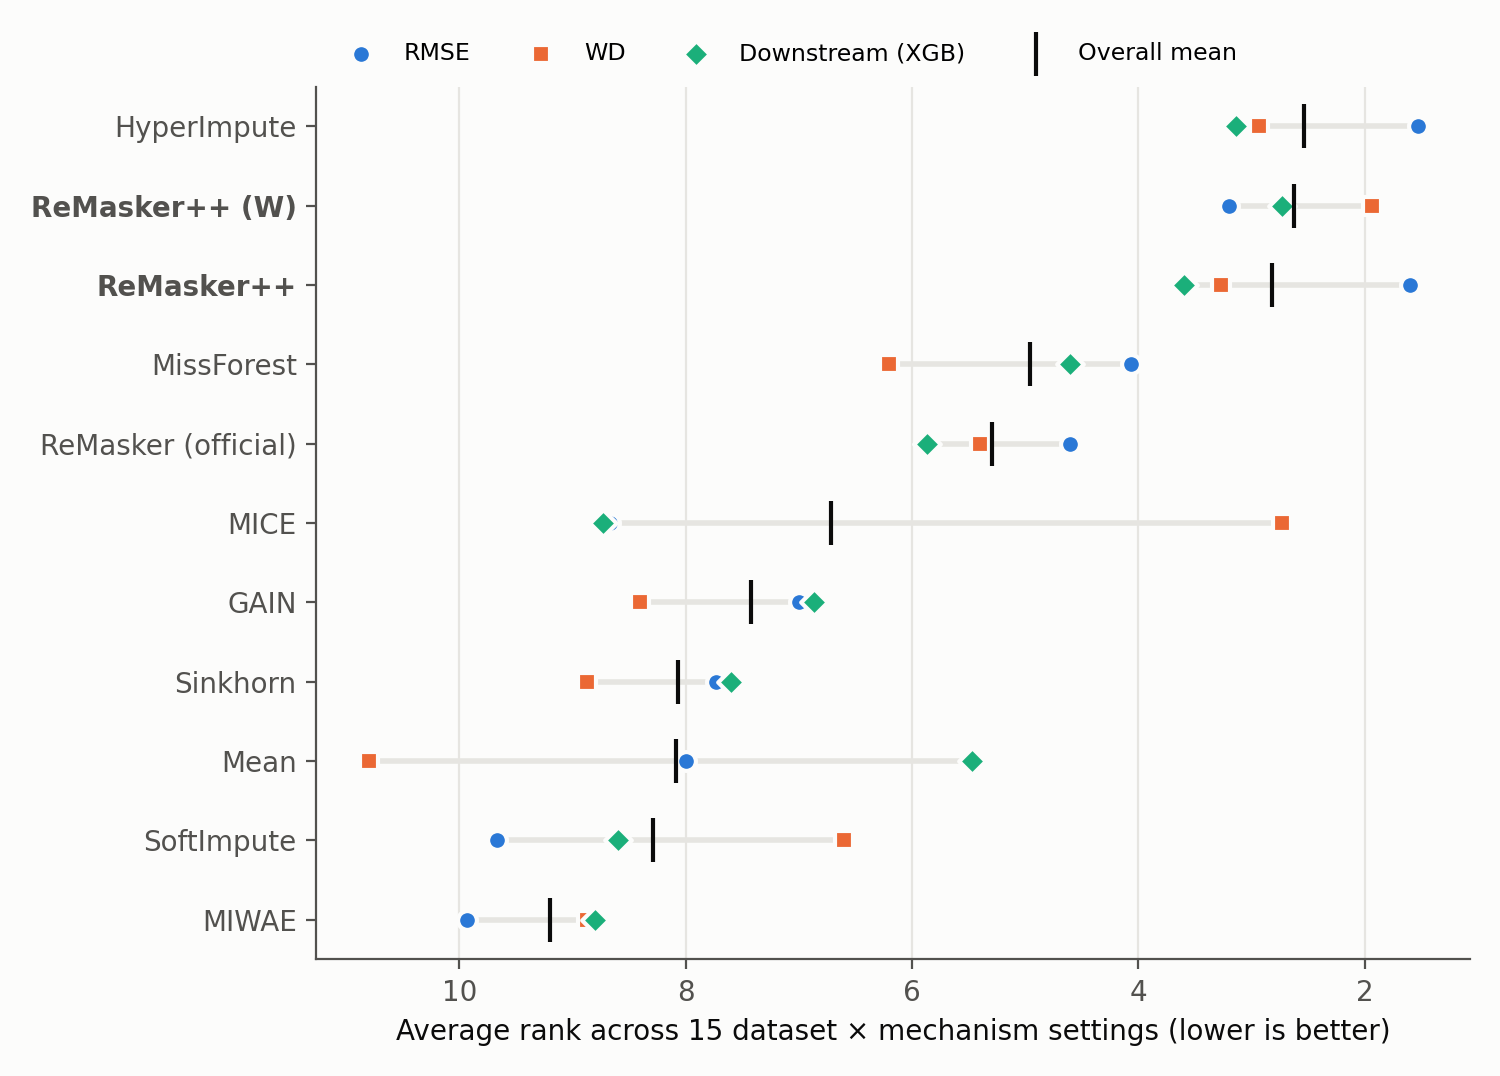
\includegraphics[height=0.8\textheight]{avg_rank.png}
\end{frame}

\begin{frame}{New capability: knowing which imputations to trust}
\begin{columns}[c]
\column{0.58\textwidth}
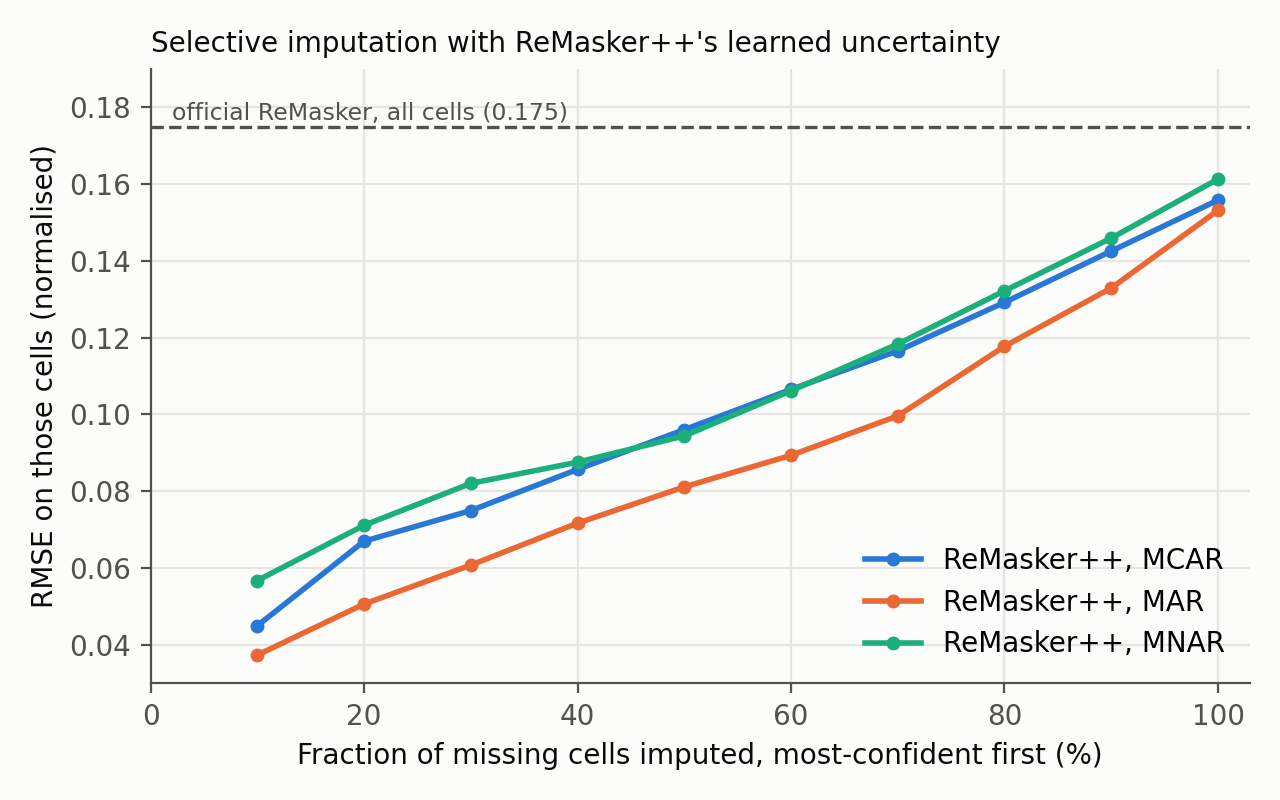
\includegraphics[width=\linewidth]{coverage_curve.png}
\column{0.4\textwidth}
\small
\begin{tabular}{lc}
\toprule
& Spearman $\rho$ \\\midrule
MC re-masking & 0.17 \\
\alert{Learned head} & \alert{0.47}\\\bottomrule
\end{tabular}\\[8pt]
25\% most confident cells:\\ RMSE \alert{0.067}\\[3pt]
25\% least confident cells:\\ RMSE 0.232 (\alert{$3.5\times$})\\[6pt]
Accept the most confident 50\%: about 40\% lower error than the full set.
\end{columns}
\end{frame}

\begin{frame}{Downstream utility}
\begin{columns}[c]
\column{0.58\textwidth}
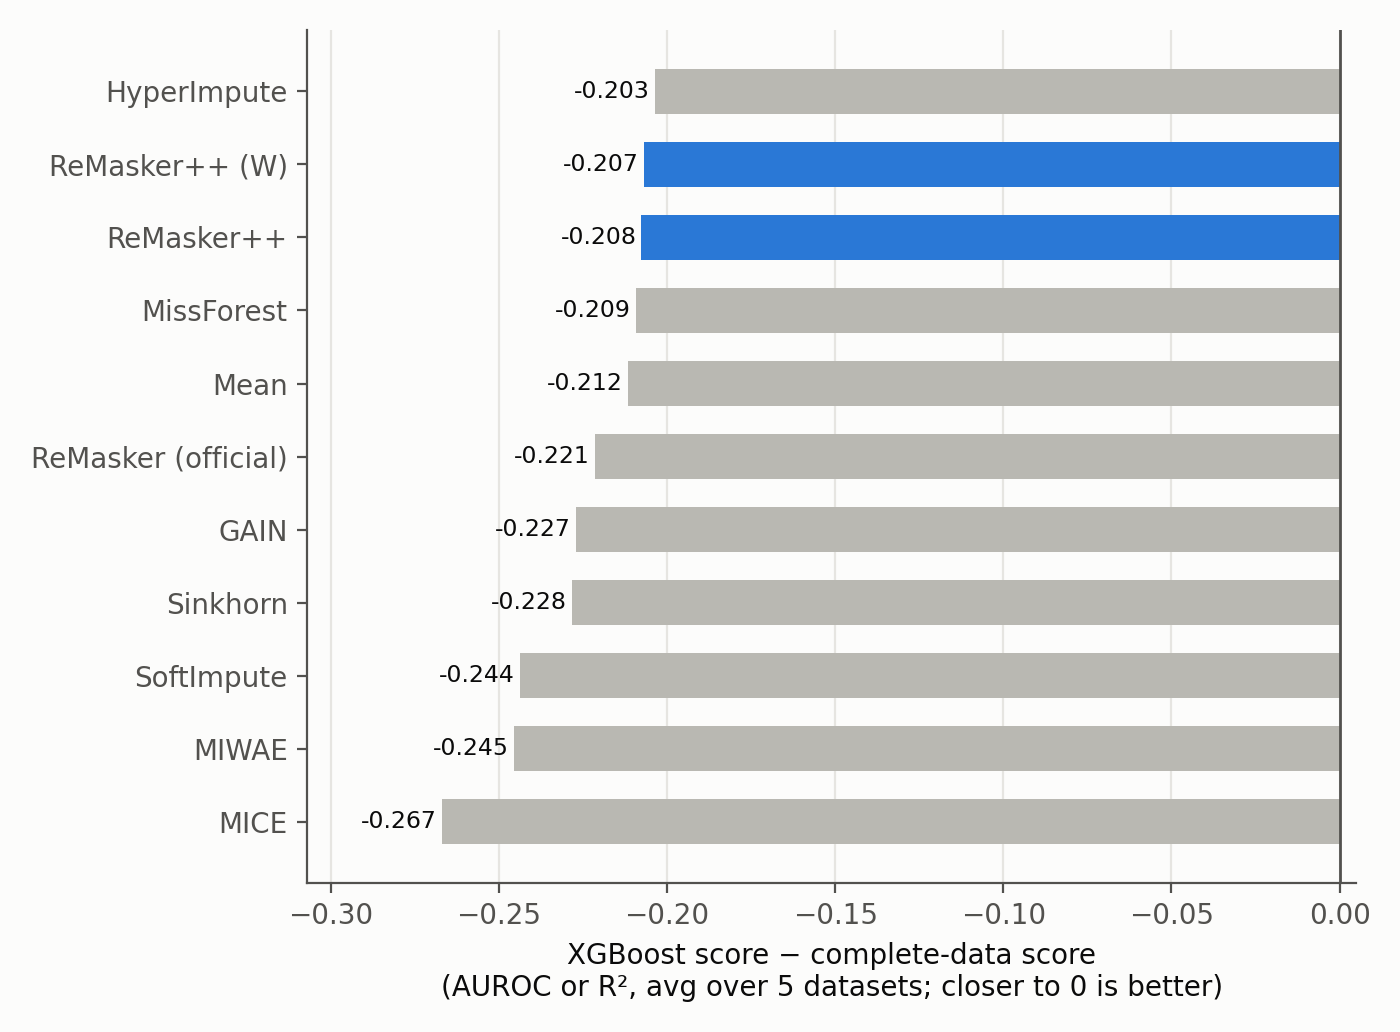
\includegraphics[width=\linewidth]{downstream_gap.png}
\column{0.4\textwidth}
\small
\begin{itemize}
\item Gap to the complete-data oracle (XGBoost): \rmpp{} $-0.207$ vs.\ ReMasker $-0.221$.
\item \rmpp{}\,(W): \alert{best average downstream rank} (2.73); beats HyperImpute in 9/15 settings.
\item Top methods lie within 0.006 of each other. Mean imputation is surprisingly good for XGBoost, so fidelity $\neq$ utility.
\end{itemize}
\end{columns}
\end{frame}

\begin{frame}{Stress test: MNAR with heavy missingness}
\centering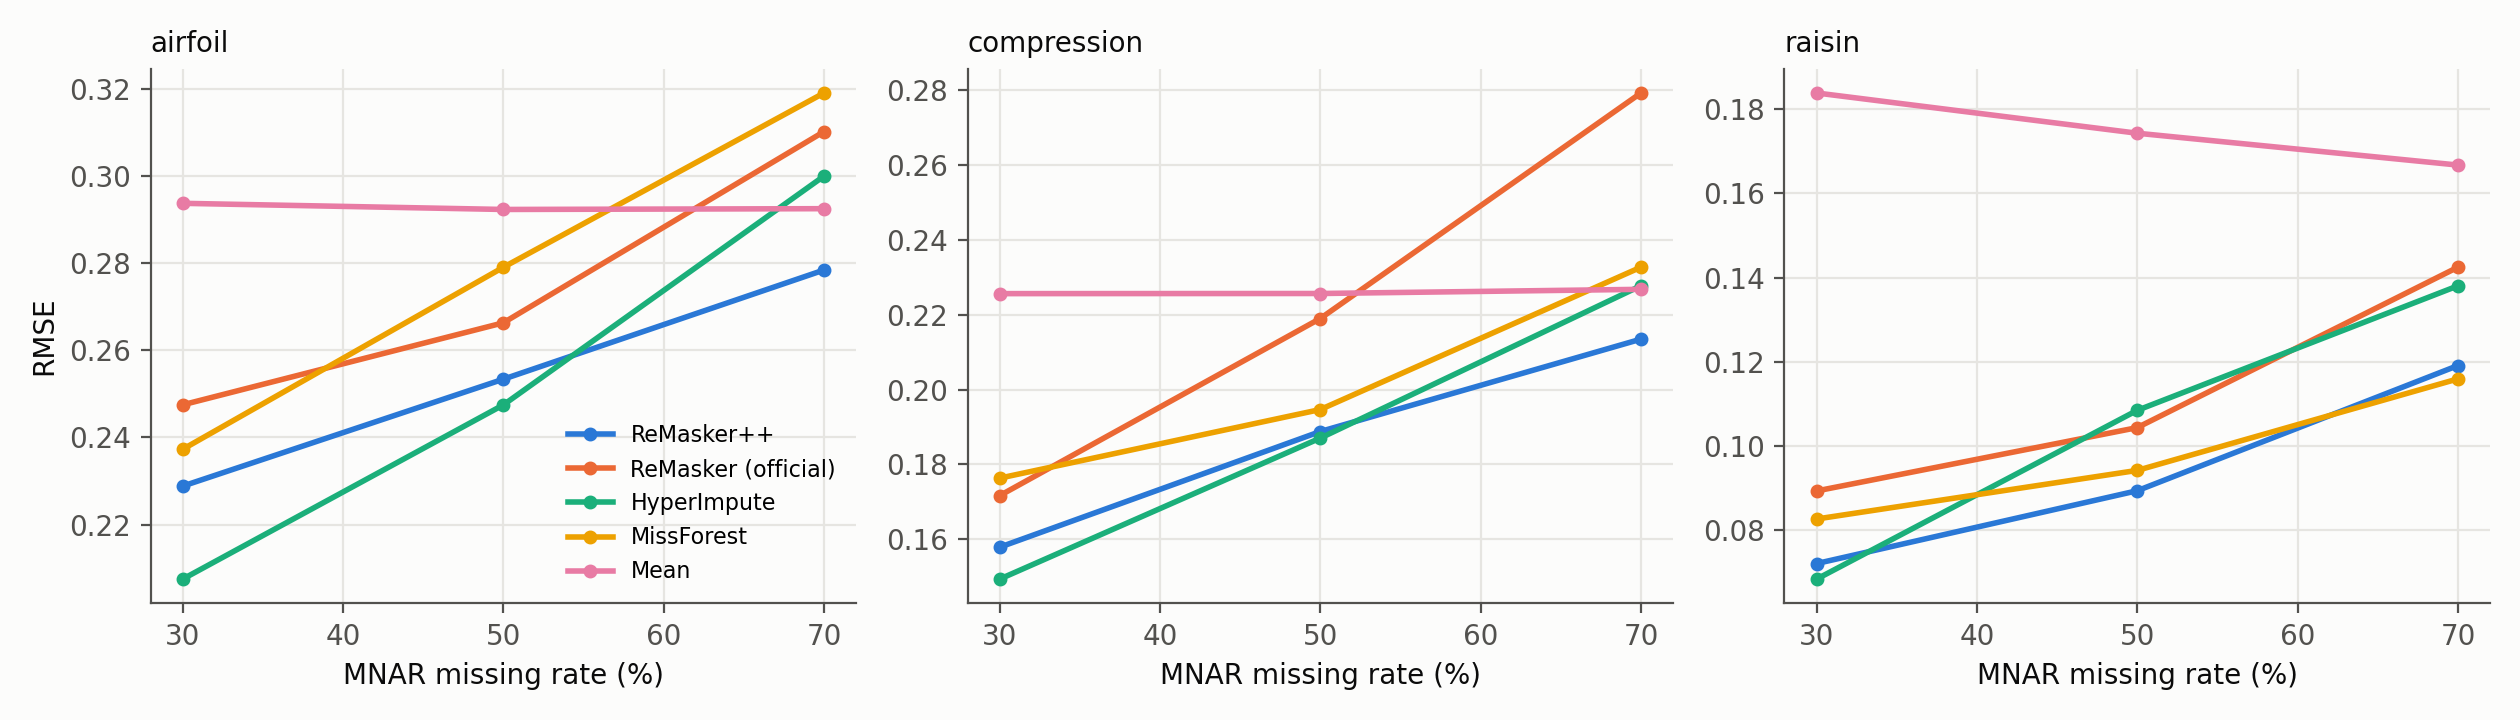
\includegraphics[width=\linewidth]{stress_mnar.png}\\
\small At 50\% and 70\% MNAR, \alert{\rmpp{} has the lowest average RMSE of all methods}. At 70\%: 0.204 vs.\ HyperImpute 0.222 ($-8\%$) and ReMasker 0.244 ($-17\%$).
\end{frame}

\begin{frame}{Honest negatives \& limitations}
\textbf{What did not work (in the ablation):}
\begin{itemize}
\item Missingness-pattern embedding: overfits, +18\% RMSE.
\item MC re-masking uncertainty: barely correlated with error ($\rho\approx0.17$); the learned head is far better.
\item Uncertainty-guided progressive imputation: worse than one-shot.
\end{itemize}
\textbf{Limitations:} CPU budget (4000 steps, 5 datasets, 3 seeds); CACTI / DiffPuter / TabImpute not re-run; numerical features only.
\end{frame}

\begin{frame}{Conclusion}
\begin{itemize}
\item \rmpp{} = ReMasker + \alert{missingness-aligned re-masking} + \alert{learned uncertainty} (+ Wasserstein loss).
\item vs.\ ReMasker: \alert{$-11.5\%$ RMSE, $-25\%$ WD}, better in 15/15 settings; average rank 5.3 $\to$ 2.6--2.8.
\item Level with HyperImpute overall (rank 2.53); \alert{best WD and downstream rank}; \alert{best under heavy MNAR}.
\item \alert{New capability}: calibrated per-cell confidence for selective imputation.
\item Future: multiple imputation from the uncertainty, learned masking for MNAR, categorical data, comparison with CACTI / DiffPuter / TabImpute.
\end{itemize}
\end{frame}

\begin{frame}[standout]
Thank you! Questions?\\[6pt]
\normalsize\texttt{github.com/sunno-bhaato/remasker\_pp}
\end{frame}
\end{document}
